%!TEX root=../document.tex
\section{Ergebnis}
\label{sec:Ergebnis}

Folgende Punkte wurden bearbeitet:

\begin{itemize}
	\item Allgemein
	\item CherryPy und andere angewendeten Technologien
	\item Umsetzung
	\item Aufgetretene Probleme	
	\item Ergebnis
\end{itemize}

\subsection{Allgemein}

Wir haben uns für CherryPy entschieden und für einen Anwendungsfall, der schnell zu implementieren und eine niedrige Komplexität aufweist. Das ist laut CherryPy einer der häufigsten Anwendungsfälle für CherryPy. Ein weiterer wichtiger Vorteil ist, dass CherryPy auf OOP ausgelegt ist und lässt sich dadurch zusätzlich leichter schreiben und verstehen.

Wir haben eine Webseite mit CRUD-Funktionen erstellt mit denen man Benutzer verwalten kann. 
Dazu haben wir in der Datenbank eine Tabelle angelegt die wie folgt ausschaut:

\begin{figure}[H]
	\centering
	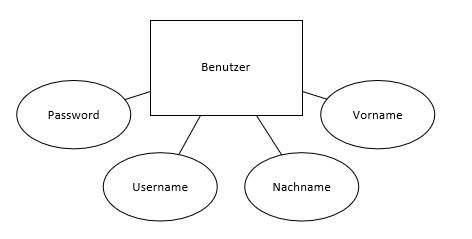
\includegraphics[width=0.5\linewidth]{images/db}
	\caption{Aufbau von Benutzer}
	\label{fig:Benutzeraufbau}
\end{figure}


Das Einsteigen in CherryPy ist mit Abstand einer der größten Vorteil, den mit wenigen Zeilen lässt sich eine Webseite erstellen und bereitstellen.
\begin{lstlisting}[language=Python]
import cherrypy

class HelloWorld(object):
	@cherrypy.expose
	def index(self):
		return "Hello World!"

cherrypy.quickstart(HelloWorld())
\end{lstlisting}

Mit diesen Zeilen ist eine Webseite erstellt und funktionsfähig

Insgesamt beläuft sich der Arbeitsaufwand auf ungefähr \textbf{10 Stunden}.

\subsection{CherryPy und andere angewendeten Technologien}

CherryPy ist ein Non-Full-Stack-Framework und bietet mit einer sehr einfachen Verfahren einen Webserver an, der mit wenigen Befehlen gestartet und mit Inhalt gefüllt werden kann.

Weiters haben wir für unsere Persistierung die eingebaute Schnittstelle von Python zu SQLite verwendet. Dieses Schnittstelle ermöglicht es mit wenigen Befehlen eine simple Datenbank zu betreiben. Allerdings hatten wir auch einigen Probleme mit der Datenbank auf die wir später noch genauer eingehen.

Um die Webseite mit der CherryPy-Rückgaben zu verbinden, haben wir jQuery verwendet. 

Zusätzlich haben wir, um der Webseite ein sprechenden Design zu geben, CSS und Bootstrap verwendet. 


\subsection{Umsetzung}


Die Übung ist in 2 Bereiche aufzuteilen, den Server Teil, dieser kümmert sich um das Speichern und Lesen aus der Datenbank, diese Aufgabe wurde mittels den Python WebFramework CherryPy umgesetzt. Der Client Teil kümmert sich hingegen um die Darstellung sowie um die Eingaben, dies wurde mittels HTML, CSS und JavaScript umgesetzt.

\subsubsection{CherryPy}

Als erstes wurde eine Klasse CRUD erstellt, diese wird aufgerufen sobald man auf localhost mit der entsprechenden Port Nummer zugreift. Die Klasse öffnet die index.html Datei und sendet den Inhalt an den Browser zurück.

\begin{lstlisting}[language=Python, caption=Klasse zur Darstellung der Index.html]
class CRUD(object):
	@cherrypy.expose
	def index(self):
		return open('index.html')
\end{lstlisting}

Nun wurde eine Klasse erstellt, welche auf die HTML Befehle reagiert, dies sind GET, POST, PUT, ... . In unserem Fall haben wir nur POST verwendet mit 2 Parameter. Der erste Parameter param gibt an welche Aktion wir durchführen wollen, der zweite Parameter input gibt liefert zusätzliche Informationen, wie zum Beispiel eingeben Werte.

\begin{lstlisting}[language=Python, caption=Klasse zur verwaltung der HTML Befehle]
@cherrypy.expose
class CRUDWebService(object):

	@cherrypy.tools.accept(media='text/plain')
	def POST(self, param, input):
\end{lstlisting}

Wird ein read als Parameter gesendet, erwartet sich der Client alle Benutzer. Aus diesem Grund werden alle Benutzer aus der Datenbank ausgelesen und eine HTML Tabelle erstellt. Diese wird dann als HTML Response zum Client zurückgesendet und dargestellt.

\begin{lstlisting}[language=Python, caption=Auslesen aller Benutzer aus der Datenbank]
if param == "read":
	with sqlite3.connect(DB_STRING) as c:
		r = c.execute("SELECT * FROM benutzer")
		response = "<table width='100%' class='table table-striped table-bordered'" \
		"cellspacing='0'><tr><td>Nr</td><td>Vorname</td><td>Nachname</td>" \
		"<td>Username</td></tr>"
		while True:
			row = r.fetchone()
			if row is None:
				break
			response += "<tr><td>" + str(row[0]) + "</td><td>" + row[1] + "</td><td>" + row[2] + 		"</td><td>" + row[3] + "</td></tr>"
		response += "</table>"
	return response
\end{lstlisting}

Auf den Parameter update reagiert das Programm sehr ähnlich, einziger Unterschied ist, dass die Benutzer in einer Tabelle zurückgeliefert werden, die bei jedem Benutzer einen Button zum Bearbeiten hat. Außerdem müsste hier ein kurzes sleep eingebaut werden, da update gleich nach einer Datenbank ändern die neuen Benutzer ausliest, dadurch konnte es passieren das beim Auslesen noch nicht die neuen Werte dabei waren.

\begin{lstlisting}[language=Python, caption=Auslesen aller Benutzer aus der Datenbank und bearbeitbar zurückliefern]
if param == "update":
	sleep(0.05)
	with sqlite3.connect(DB_STRING) as c:
		r = c.execute("SELECT * FROM benutzer")
		response = "<table width='100%' class='table table-striped table-bordered'" \
		"cellspacing='0'><tr><td>Nr</td><td>Vorname</td><td>Nachname</td>" \
		"<td>Username</td><td>Aendern</td></tr>"
		while True:
			row = r.fetchone()
			if row is None:
				break
			response += "<tr><td>" + str(row[0]) + "</td><td>" + row[1] + "</td><td>" + row[2] + "</td><td>" + row[3] + "</td><td> <button onClick='updateBenutzer(" + str(row[0]) + ")'>Aendern</button></td></tr>"
		response += '</table>'
	return response
\end{lstlisting}

Wenn der Benutzer eine Person bearbeiten will, müssen die aktuellen Informationen von dieser Person abgerufen werden, hierfür gibt es den Parameter getBenutzer. Dieser hat zusätzlich als input die Nummer, welche der Primary Key der Entität ist. Die zurückgelieferten Informationen werden, dann in Input Felder angezeigt um diese zu bearbeiten.

\begin{lstlisting}[language=Python, caption=Auslesen eines Benutzer aus der Datenbank]
if param == "getBenutzer":
	with sqlite3.connect(DB_STRING) as c:
		r = c.execute("SELECT * FROM benutzer WHERE nr=" + input)
		while True:
			row = r.fetchone()
			if row is None:
				break
			response = str(row[0]) + "#" + row[1] + "#" + row[2] + "#" + row[3] + "#" + row[4];
	return response
\end{lstlisting}

Wenn der Benutzer die Informationen in den Input Feldern geändert hat und auf Speichern klickt, werden die neuen Informationen über den Parameter updateBenutzer und die Informationen als input an den Server gesendet. Anschließend wird der Benutzer in der Datenbank aktualisiert.

\begin{lstlisting}[language=Python, caption=Updaten der Benutzerinformationen]
if param == "updateBenutzer":
	with sqlite3.connect(DB_STRING) as c:
		liste = input.split('#')
		c.execute("UPDATE benutzer SET vorname='" + liste[1] + "',nachname='"
			+ liste[2] + "',username='" + liste[3] + "',password='" + liste[4] + "' WHERE nr=" + liste[0])
	return "Benutzer erfolgreich geaendert."
\end{lstlisting}

Wird ein neuer Benutzer erstellt, wird über den Parameter create und den Benutzerinformationen als input an den Server gesendet. Dieser speichert die Informationen in der Datenbank.

\begin{lstlisting}[language=Python, caption=Updaten der Benutzerinformationen]
if param == "create":
	with sqlite3.connect(DB_STRING) as c:
		liste = input.split('#')
		c.execute("INSERT INTO benutzer(vorname, nachname, username, password) VALUES (" + liste[0] + ", "
		+ liste[1] + ", " + liste[2] + ", " + liste[3] + ")")
	return "Benutzer erfolgreich gespeichert."
\end{lstlisting}

Der delete Branch ist sehr ähnlich zum update Branch, der einzige Unterschied ist, dass anstele eines Update Button wird ein Löschen Button erstellt.

\begin{lstlisting}[language=Python, caption=Auslesen aller Benutzer mit einen Löschen Button]
if param == "delete":
	with sqlite3.connect(DB_STRING) as c:
		r = c.execute("SELECT * FROM benutzer")
		response = "<table width='100%' class='table table-striped table-bordered'" \
					"cellspacing='0'><tr><td>Nr</td><td>Vorname</td><td>Nachname</td>" \
					"<td>Username</td><td>Loeschen</td></tr>"
		while True:
			row = r.fetchone()
			if row is None:
				break
			response += "<tr><td>" + str(row[0]) + "</td><td>" + row[1] + "</td><td>" + row[2] + "</td><td>" \
			+ row[3] + "</td><td> <button onClick='deleteBenutzer(" + str(row[0]) + ")'>Loeschen" \
			"</button></td></tr>"
		response += '</table>'
	return response
\end{lstlisting}	

Abschließend können Benutzer aus der Datenbank gelöscht werden, hierfür wird als Parameter deleteBenutzer angegeben und als input die Nummer des Benutzers. Falls ein ungültiger Parameter gesendet wird, wird ein error zurückgeliefert.

\begin{lstlisting}[language=Python, caption=Löschen eines bestimmten Benutzers]
if param == "deleteBenutzer":
	with sqlite3.connect(DB_STRING) as c:
		c.execute("DELETE FROM benutzer WHERE nr=" + input)
	return self.POST("delete", "")

return "Ungueltige Anfrage"
\end{lstlisting}

Weiters gibt es die Methode setup\_database diese wird immer beim Starten des Servers ausgeführt und soll sicherstellen, dass die Datenbank sowie Tabelle vorhanden ist. Außerdem werden in diesem Fall noch 2 Benutzer als Testdaten standardmäßig importiert.

\begin{lstlisting}[language=Python, caption=Erstellen der Tabelle Benutzer beim Start des Servers]
def setup_database():
	with sqlite3.connect(DB_STRING) as con:
		con.execute("DROP TABLE IF EXISTS benutzer")
		con.execute("CREATE TABLE IF NOT EXISTS benutzer(nr INTEGER PRIMARY KEY AUTOINCREMENT, vorname VARCHAR, "
		"nachname VARCHAR, username VARCHAR, password VARCHAR)")
		con.execute("INSERT INTO benutzer VALUES(null,'Marvin', 'Ertl', 'mertl', 'password')")
		con.execute("INSERT INTO benutzer VALUES(null,'Lukas', 'Zuba', 'lzuba', 'password')")
\end{lstlisting}

Ebenso gibt es eine Methode namens cleanup\_database, diese löscht die Tabelle beim Beenden des Server.

\begin{lstlisting}[language=Python, caption=Löschen der Tabelle benutzer beim Beenden des Servers]
def cleanup_database():
	with sqlite3.connect(DB_STRING) as con:
		con.execute("DROP TABLE IF EXISTS benutzer")
\end{lstlisting}

Abschließend wird in einer IF-Anweisung die Konfiguration hineingeschrieben um den Server zu starten. Ebenfalls wird hier auch angegeben welche Methoden beim Starten sowie beim Beenden des Servers ausgeführt werden sollen. Außerdem wird die auto reload ausgeschaltet, dies führt ansonsten dazu, dass wenn das Python Programm abstürzt der Server weiterhin im Hintergrund den Port belegt. Schlussendlich wird angeben welche Klasse beim Aufrufen reagiert, sowie welche Klasse auf die HTML Befehle reagiert.  

\begin{lstlisting}[language=Python, caption=Konfiguration des Servers]
if __name__ == '__main__':
	conf = {
		'/': {
			'tools.sessions.on': True,
			'tools.staticdir.root': os.path.abspath(os.getcwd())
		},
		'/generator': {
			'request.dispatch': cherrypy.dispatch.MethodDispatcher(),
			'tools.response_headers.on': True,
			'tools.response_headers.headers': [('Content-Type', 'text/plain')],
		},
		'/static': {
			'tools.staticdir.on': True,
			'tools.staticdir.dir': './public'
		}
	}
	cherrypy.engine.subscribe('start', setup_database)
	cherrypy.engine.subscribe('stop', cleanup_database)
	cherrypy.config.update({'server.socket_port': 8080})
	cherrypy.config.update({'engine.autoreload_on': False})
	
	webapp = CRUD()
	webapp.generator = CRUDWebService()
	cherrypy.quickstart(webapp, '/', conf)
\end{lstlisting}

\subsubsection{HTML}

Bei der index.html Datei handelt es sich um eine einfache Webseite welche mittels Bootstrap gestaltet worden ist. Auf den HTML Teil wird hier nicht genauer eingegangen, da es sich bei diesem um ein paar Tabellen sowie input Felder und Button mit ein bisschen CSS Formatierung handelt.

Viel wichtiger ist der JavaScript Teil, dieser ließt nämlich die Eingaben aus und sendet diese an den Server.

Nachfolgend ist der JavaScript Code, welcher Aufgerufen wird, wenn der Button showRead angeklickt wird. Als erstes werden alle anderen Tabs geschlossen und anschließend über die Post Methode mittels den Parameter read eine Anfrage gesendet. Als Response kommt die Tabelle mit allen Benutzer zurück, diese wird an bei dem Element listBenutzer eingefügt.

\begin{lstlisting}[language=HTML, caption=Anfrage senden an den Server]
$("#showRead").click(function(e) {
	closeTabs();
	$.post("/generator", {"param": "read", "input": ""})
	.done(function (string) {
		$("#read-string").show();
		document.getElementById("listBenutzer").innerHTML = string;
	})
	e.preventDefault();
});
\end{lstlisting}

Die restlichen Methoden für die anderen Funktionen sind gleich aufgebaut, einige überprüfen die Eingaben davor noch bzw. fassen die Angaben zu einen String zusammen, welcher anschließend als String über die input Variable an den Server gesendet wird.

Ansonsten wurde noch ein bisschen JavaScript verwendet um, Eingabemöglichkeiten zu verstecken bzw. anzuzeigen wenn diese benötigt werden. Dadurch wird die Oberfläche übersichtlicher und einfacher bedienbar.

\subsection{Aufgetretene Probleme}

\subsubsection{Tabelle nicht gefunden}
Die häufigste Fehlermeldung dieser Art war: $ no\,such\,table:\,benutzer $ 

Diesen Fehler konnten wir auf keine genaue Stelle eingrenzen, da dieser Fehler zufällig beim Starten des Server hin und wieder aufgetreten ist. 

Gelöst haben wir diesen Fehler dann durch das Sicherstellen, dass die Tabelle noch existiert und wenn nicht die Tabelle neu erstellt und mit Standarddatensätzen wieder befüllt wird.

\subsubsection{Datensatz nicht richtig abgespeichert}
Ein Fehler, der leicht zu lösen war, war: $ no\,such\,attribute:\,zuba $ 

Hierbei hat es sich um eine INSERT Anweisung gehandelt, die eine syntaktisch falschen Aufbau hatte, den wir allerdings erst sehr spät bemerkt haben. 

Gelöst haben wird dies, indem wir die Zusammensetzung der Anweisung neu geschrieben haben und explizit die Reihenfolge der Attribute angegeben haben.

\subsubsection{JS Funktionen nicht aufrufbar}
Ein nicht so einfach findbarer Fehler war, $ function\,showuser\,not\,found $ 

Bei diesem Fehler wurde eine Anfrage an den Server gesendet, durch einen Syntax Fehler bzw. dadurch das es lange her ist, seit wir mit JavaScript gearbeitet haben, gab es einen Fehler beim Absenden der Anfrage. Da aber die Anfrage gesendet worden ist, haben wir den Fehler erst am Server gesucht, da dort der Fehler auch aufgetreten ist, dabei war aber die gesendete Anfrage nicht im richtigen Format.


\subsection{Ergebnis}


Das Ergebnis der Übung ist eine Webseite, die die CRUD Funktionen bereitstellt, um Benutzer zu verwalten.

CREATE:
\begin{figure}[H]
	\centering
	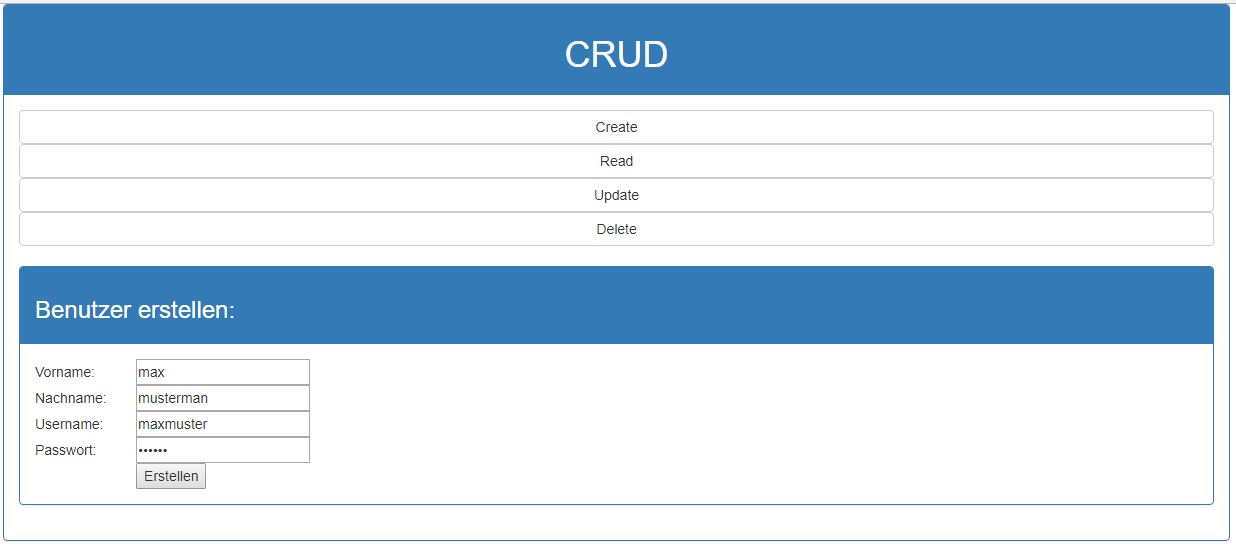
\includegraphics[width=1\linewidth]{images/create}
	\caption{CREATE Funktion}
	\label{fig:create}
\end{figure}

READ:
\begin{figure}[H]
	\centering
	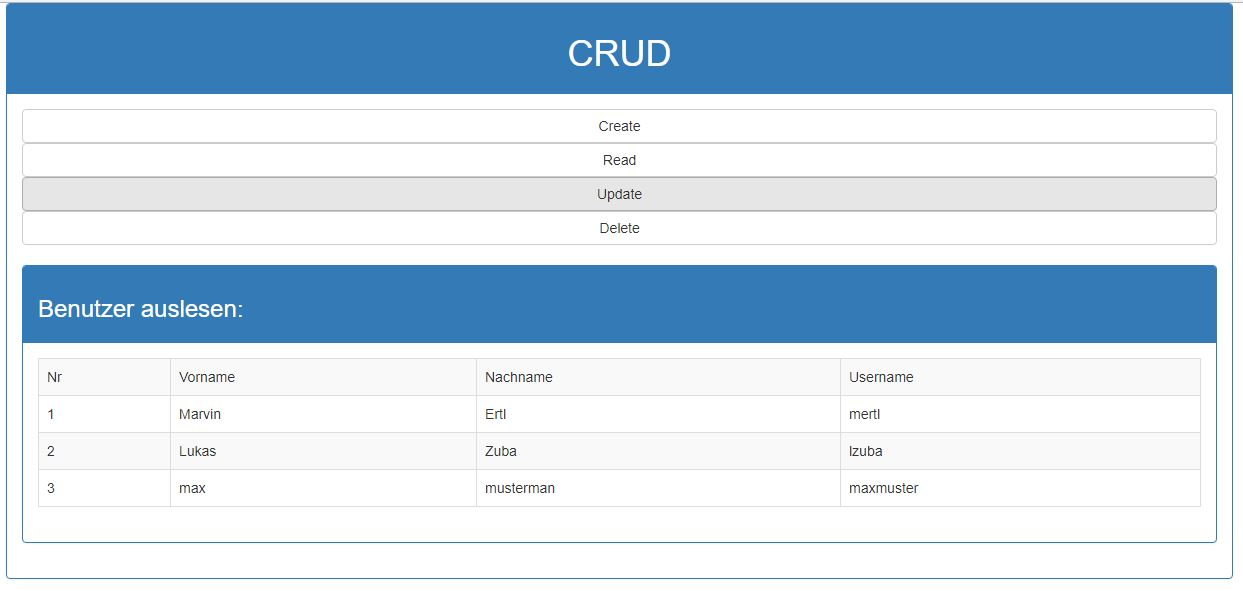
\includegraphics[width=0.9\linewidth]{images/read}
	\caption{READ Funktion}
	\label{fig:read}
\end{figure}

UPDATE:
\begin{figure}[H]
	\centering
	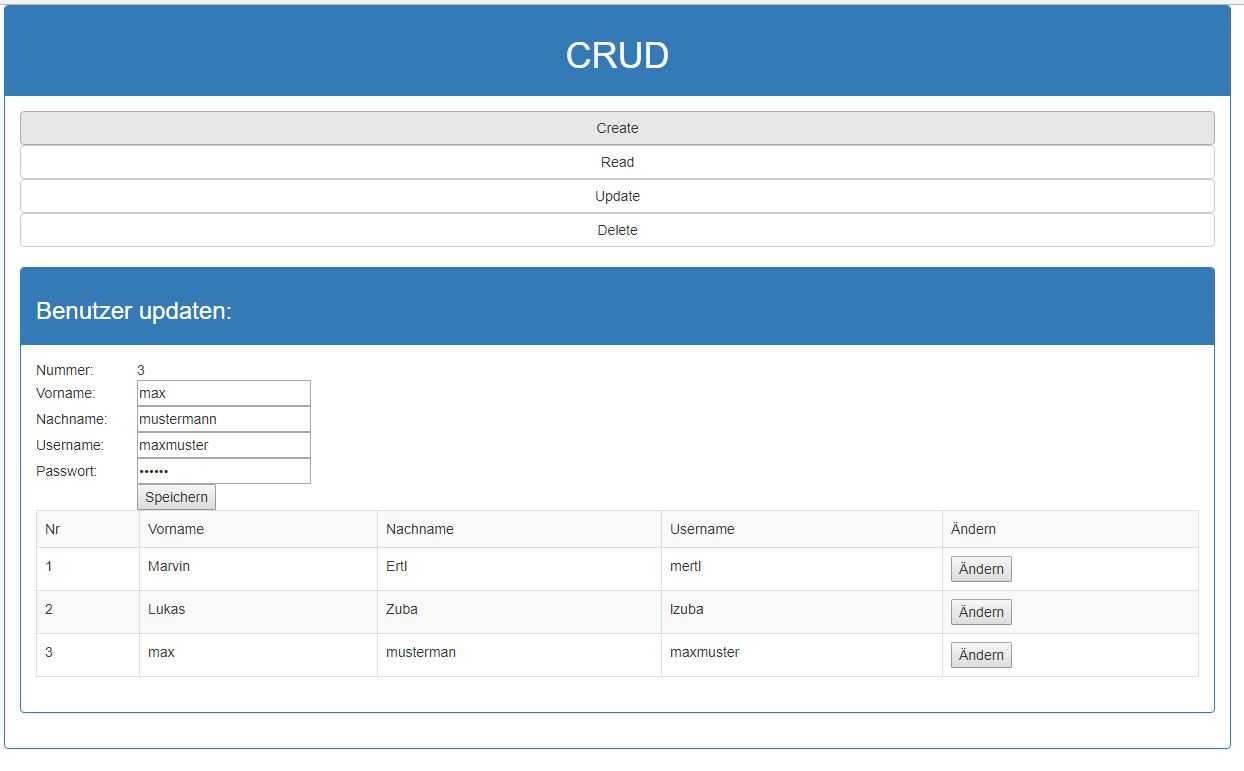
\includegraphics[width=0.9\linewidth]{images/update}
	\caption{UPDATE Funktion}
	\label{fig:update}
\end{figure}

DELETE:
\begin{figure}[H]
	\centering
	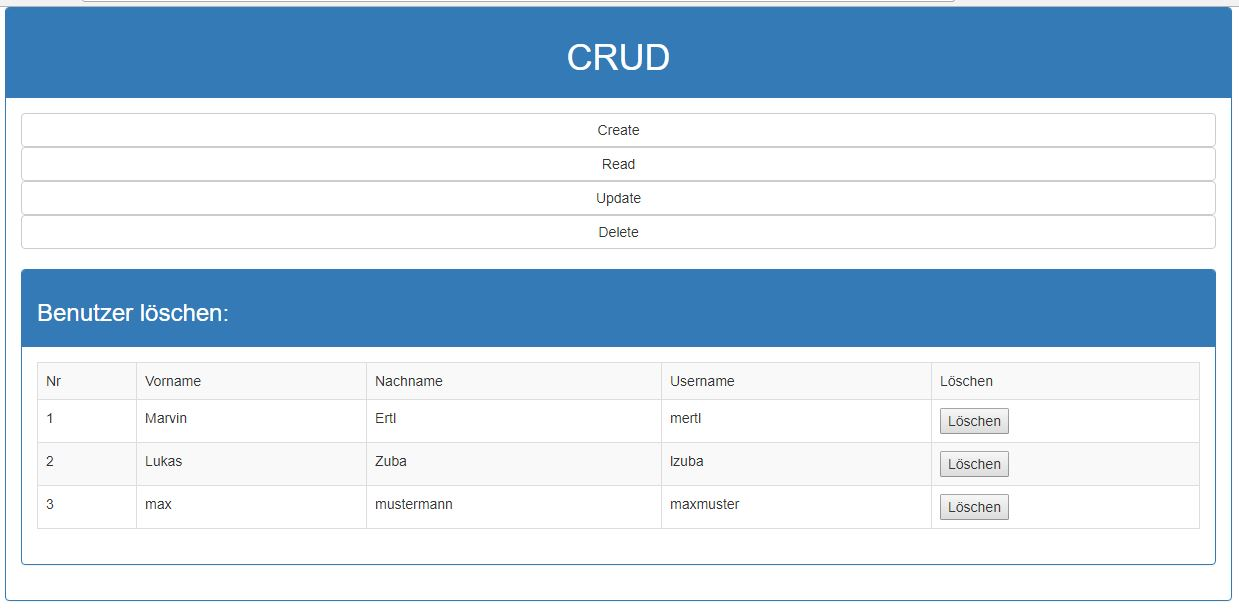
\includegraphics[width=1\linewidth]{images/delete}
	\caption{DELETE Funktion}
	\label{fig:delete}
\end{figure}

\begin{figure}[H]
	\centering
	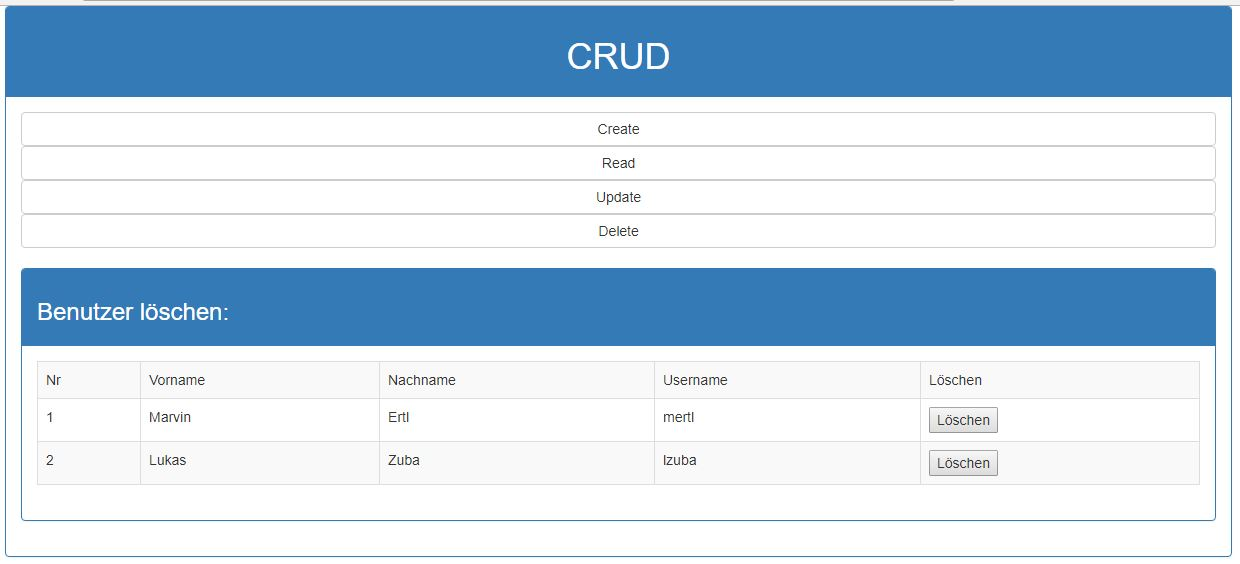
\includegraphics[width=1\linewidth]{images/delete_after}
	\caption{DELETE nach dem Löschen von Max Mustermann}
	\label{fig:deleteafter}
\end{figure}
